\documentclass[11pt,letterpaper,boxed]{pset}

\usepackage[margin=0.75in]{geometry}
\usepackage{ulem}

\name{Name: \rule{2.5cm}{0.15mm}}
\assignment{Box \# \rule{1.5cm}{0.15mm}}
\class{MATH060 HW8}

\begin{document}

    \problemlist{MATH060 HW8}
    \begin{center}
    	5.2: 7, 14\\
    	5.3: 1, 13, 18\\
    \end{center}
    
    \begin{problem} [5.2.7]
    	Evaluate the given iterated integrals. In addition, sketch the regions D that are determined by the limits of integration.
    
    	\[\int_{-1}^{3} \int_{x}^{2x+1} xy \textrm{ } dy dx\]
    \end{problem}
    \newpage
    
    
    \begin{problem} [5.2.14]
    	The figure below shows the level curves indicating the varying depth (in feet) of a 25 ft by 50 ft swimming pool. Use a Riemann sum to estimate, to the nearest 100 ft$^3$, the volume of water that the pool contains.
    \end{problem}
    
    \begin{figure} [h!]
            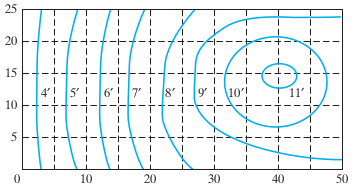
\includegraphics[width=90mm]{pool.png}
    \end{figure}
    \newpage
    
    
    \begin{problem} [5.3.1]
    	Consider the integral
    
    	\[\int_{0}^{2} \int_{x^2}^{2x} (2x + 1) dydx\]
    	
    	\begin{enumerate}
    	    \item Evaluate this integral.
    	    \item Sketch the region of integration.
    	    \item Write an equivalent iterated integral with the order of integration reversed. Evaluate this new integral and check that your answer agrees with part (a).
    	\end{enumerate}
    	
    \end{problem}
    \newpage
    
    
    \begin{problem} [5.3.13]
    	Rewrite the given sum of iterated integrals as a single iterated integral by reversing the order of integration, and evaluate.
    
    	\[\int_{0}^{8} \int_{0}^{\sqrt{y/3}} y \textrm{ } dxdy +
    		\int_{8}^{12} \int_{\sqrt{y-8}}^{\sqrt{y/3}} y \textrm{ } dxdy \]
    \end{problem}
    \newpage
    
    
    \begin{problem} [5.3.18]
    	Evaluate the given iterated integral.
    	\[\int_{0}^{2} \int_{y/2}^{1} e^{-x^2} dxdy\]
    \end{problem}
    \newpage
    
\end{document}